\section{Results}\label{sec:results}

To guide the research and operationalize the interview survey %and to help the identification of the findings needed to answer the research questions 
we carefully formulated a set of propositions that are then confirmed or negated by analysing the data collected through the semi-structured interviews we performed. Specifically, the first four propositions are defined for RQ1, propositions  5 and 6 are defined for RQ2,  and the remaining two are defined for RQ3.
The propositions aim at helping eliciting the different facets of transparency and contract-based collaborations and are based on knowledge that we acquired in numerous meetings we had with Volvo Cars and many suppliers within the NGEA and NGEA2 projects, and in our multi-annual and established collaboration with these companies. % and also on the result of literature review done
%prior to this research and are mapped as follows to the research questions: 

%\begin{table}[htb]
%\centering
%\begin{tabular}{|c|c|}\hline
%{\bf Research Question 1} & {\bf Research Question 2} \\ \hline % & {\bf Res. Quest. 4}\\ \hline
%		 &   \\ \hline
%		 & 	  \\ \hline
%		 &    \\ \hline
%		 &    \\ \hline
%		 & 	  \\ \hline		
%\end{tabular}
%\caption{Mapping propositions to research questions}
%\label{tab:mappingProRQs}
%\vspace{-.4cm}
%\end{table}


In Section~\ref{sec:ResearchQuestion1} we present findings related to research question 1, in Section~\ref{sec:ResearchQuestion2} we present findings related to research question 2,  in Section~\ref{sec:ResearchQuestion3} we present findings related to research question 3, and finally
 in Section~\ref{sec:findings_RQs} we summarize the main findings and challenges.

\subsection{Research Question 1}\label{sec:ResearchQuestion1}

The propositions we defined for  
RQ1 (i.e. {\em What are the risks and/or benefits of increasing inter-organisational transparency?}) focus on these aspects:

\begin{itemize}
\item {\em Transparency is a necessary condition for  inter-organisational CI\&D} - Proposition 1 %: Increasing inter-organisational transparency of information is a necessary condition for inter-organisational CI\&D
\item {\em Transparency is perceived positively/negatively within the companies} - Proposition 2 %: Increased inter-organisational transparency of information is considered positive
\item {\em It is easy to improve transparency} - Proposition 3 %: Inter-organisational sharing of information is considered simple between members of the projects
\item {\em There is a connection between transparency and quality of results of the project} - Proposition 4 %: A more open transparency policy improves the quality of the project and its results.
\end{itemize}

\vspace{.2cm}
\subsubsection{Proposition 1: Increasing inter-organisational transparency of information is a necessary condition for inter-organisational CI\&D}

%This proposition states that information transparency across companies is necessary for inter-organisational CI\&D. 
The interviewees were asked how important inter-organisational transparency is for CI\&D and whether it is a necessity to pursue. 
%During this research, we assumed inter-organisational transparency was a key factor for CI\&D processes across companies. However, t
The interview results {\bf reject the proposition}. Inter-organisational transparency has been identified as very important to pursue in general, but not a necessity for inter-organisational CI\&D. This answer to proposition 1 derives from the following findings.

%\rog{
%if you ask the interviewees directly they will in general say that CI\&D and transparency are two separate things, however, is this the case, look at this quotes below (can we really reject the proposition?). It might be that one can have successful project CI\&D without transparency, but from the quote below, I read that it work even better with the combination. One of these quotes can be good to include as well?
%
%Question: How important cross-organizational transparency on CI\&D?
%
%Quote: “I think it is very important, very important in general to increase efficiency. Very much for CI\&D. These two are integrated as often as possible, then smaller issues will be erased on daily basis and another main concern is when an issue arise that we need to resolve quickly. I think when you need transparency, so we can take quick decision across organizations. Without transparency decision and discussion can take too long time.”
%
%
%Here is another one I think relate to transparency:
%
%Quote: “If you don’t have the transparency into the planning status. Then it would be very difficult for Volvo to know what they can expect. Even if you separate this, I still think that it is important for the recipient to know what they are about to get in to. If they don’t have this information beforehand, how can they plan their acceptance testing. “
%
%Here is third one:
%
%Quote: “if there is a problem in specifications, we will discuss this immediately. And if that change in specification does not really impact the amount of work, nor have any business impact then the specification will be updated.”
%
%}
%\rog{There are a few quote such as 
%Quote: "I have worked that do CI without full transparency and it worked fine". 
%}
%\pat{Rob, please find a quotation saying that transparency is not necessary condition for CI\&D ?}
\noindent {\bf F1.1: Important, but not necessary.} The interviewees agree that %transparency is important but not necessary for having inter-organisational CI\&D:
information transparency and inter-organisational CI\&D are related, %integrated as often as possible, 
but also independent and successful as such, e.g. inter-organisational CI\&D without full transparency: 
%the two topics together (information transparency and inter-organisational CI\&D) are indeed important, but not necessary: 

\begin{aquote}{Project manager RFQ project, Volvo Cars}
 Transparency is super important, but not deeply related to CI\&D. [...] I don't find the logic relationship  between the topics [...] %, companies can have different concept of transparency, but still have a good CI\&D with each other.
\end{aquote}

%These two topics are related, %integrated as often as possible, 
%but also independent and successful as such, e.g. inter-organisational CI\&D without full transparency. 
In any case interviewees highlight the importance of transparency, see for instance:

\begin{aquote}{Software developer, Volvo Cars}
I think it [transparency] is very important, very important in general to increase efficiency. Very much for CI\&D. 
%These two are integrated as often as possible, then smaller issues will be erased on daily basis and another main concern is when an issue arise that we need to resolve quickly. I think when you need transparency, so we can take quick decision across organizations. Without transparency decision and discussion can take too long time.
\end{aquote}
%\pat{Rogardt, who said that? Rob, might you please add also a table presenting our population? Possible table: column with incremental number, company (Volvo cars or supplier), Role, Years of experience. The table should be in the interviewing phase of Section III}
%\rog{Volvo, Quote: "I am working as an electrical system architect. It is about software architecture on a complete vehicle level". He has been active in this role 2.5 years, and been active in this type of industry for 19 years (I think he mean Volvo, both as an employee and as a consult }

\noindent {\bf F1.2: Beneficial for synergy.} The interviewees agree that the combination of inter-organisational transparency and CI\&D produce synergy effects in terms of efficiency, trust, and mutual understanding.

\vspace{.2cm}
\subsubsection{Proposition 2: Increased inter-organisational transparency of information is considered positive}

Increasing inter-organisational transparency can be perceived differently by different stakeholders. The interviewees were asked how they considered the increase of transparency across companies, and how they perceived business and personal relationships between companies. The complexity of the project is experienced as an impediment working against full transparency of information.
However, it is not always easy to understand how to manage the new information:

\begin{aquote}{Product Owner, Tier-1 supplier}
 [...] when you are completely transparent you also have to treat that information in a sensitive way.
\end{aquote}

The interview results {\bf support the proposition}: the increase of information transparency is generally considered positive. This answer to proposition 2 is deduced from the following findings.

%\rog{I like to be a little bit provocative. Yes, most of the interviews agreed, but I find the challenges with too much transparency very interesting:-
%
%Question: Do you consider it is too much information?
%
%Quote: “There is a lot of information and there is a risk with this amount of information. People will jump to conclusions when they see some bad numbers somewhere or something that is not happening … I would not say it is too much. It is more an issue of understanding how to use the information they get from us and we need to communicate in a different way”
%
%Quote 2: “… it is difficult to manage to the new information. All of a sudden when you are completely transparent you also have to treat that information in a sensitive way.”
%
%Quote 3: “I think sometimes the customer he may not want to know everything. I think some things you shouldn’t know as customer, because it might create unnecessary stress.”
%
%Quote 4: “I think the dashboard is okay for this level of information, but if you go down one level maybe some technical issue the customers they shouldn’t need to know about. They will get fixed eventfully or other development situations.”
%
%I like this one:
%
%Quote 4: “When you go to a restaurant and you get your food, do you really need to know how dirty the kitchen is? If he food is okay, it is okay. It’s kind of that situation. When you start watching the chef and see if he washes his hands and you get into this where you start to wonder and worry about the chef and his qualities … Yes, I can reckon hat it can be too much information. Sometimes you don’t need to know what is happening in the kitchen.  For you own benefits and I know it sound terrible, but it is a conclusion I take sometimes you don’t need to know everything.” 
%
%Quote 5: “One thing is Intellectual Property. You transfer knowledge and software between companies and it can be tricky license wise since we are building a Linus based platform which has many different source and components.”
%}
%\pat{these are more about proposition 6, right?}
%\rog{partially, but this seem not to good: People will jump to conclusions when they see some bad numbers somewhere or something that is not happening. Off course, transparency is mostly good:-}


\noindent {\bf F2.1: Increased transparency is positive.} All the interviewees experience positively the increase of inter-organisational transparency between companies and employees, for both business and personal relationships: 

\begin{aquote}{Software developer, Volvo Cars}
%Volvo Cars could order a Linux system and get this in a traditional way. We get binary report and get the delivery at the end and we could be happy. We will lose something, because we are building this software together and we have the rights to won and use them the future. Having 
Transparency and CI\&D really give a benefit to Volvo Cars in the future reuse of assets, knowledge and experience.
\end{aquote}


The interviewees experience positive effects in terms of more awareness of the project status and increased mutual understanding. In particular, Volvo Cars employees found sharing a workplace with developers of the supplier especially effective for creating a shared mental model.  %, thanks to the closer interaction with e.g. software developers.
However, it is important to identify which kind of information should be shared. 
%\begin{aquote}{System Lead, Tier-1 supplier}
%There is a lot of information and there is a risk with this amount of information. People will jump to conclusions when they see some bad numbers somewhere or something that is not happening
%I would not say it is too much. It is more an issue of understanding how to use the information they get from us and we need to communicate in a different way".
%\end{aquote} 
As we can see there will be always some information that should not be shared:

\begin{aquote}{Chief Engineer, Tier-1 supplier}
%I would say that we nearly have full transparency. I would say transparency always goes 2 ways. Volvo Cars is also sharing with us at the same level and 
[...] they [Volvo Cars] still keep 5\% information for themselves such as business-critical information (future plans for example). But they are getting more and more open on that as well
\end{aquote}

This aspect is important also for the suppliers:

\begin{aquote}{System Lead, Tier-1 supplier}
When we are doing our estimation or calculations of our prices, this is internally done. That is the setup today. It is a fixed price project, due to that. So we are still in a traditional OEM and supplier role.
\end{aquote}

%\rog{supporting quotes 
%
%Quote 1:  “ Normally, when we work with our customer we are not allowed to share our interval bug report details. But in this project, since we have our customer in our teams, they will see that kind of information.”
% 
%Quote 2: “ When we are doing our estimation or calculations of our prices, that is internally done. That is the setup today. It is a fixed price project, due to that. So we are still in a traditional OEM and supplier role”
%
%Quote 3: “But if you compare it to other agile project that we have performed, then we have had at least one where we had a shared site and we were at the customers site. That was also good, because it was easy for the communication. I would think that in this project it is even better because we are sitting next to each other and are mixed. In the earlier project we were actually divided. We were sitting at xxx and there was a special area that was for supplier, so we were sitting there. The other area was for xxx. Even if we were sitting next to each other, it was still a little bit longer because you needed to go to their area. Rut if you are already mixed together, then type are like our colleagues.”
%
%Quote 4: “ I would say that we nearly have full transparency. I would say transparency always goes 2 ways. Volvo is also sharing with us at the same level and they still keep 5\% information for themselves such s business critical information (future plans for example). But they are getting more and more open on that as well”
%
%}

\noindent {\bf F2.2: Trust is increased.} The increase of transparency of information increases trust, too, on two levels. Firstly, increased trust between stakeholders improves collaboration and communication. Secondly, the trust gained in past projects %(thanks to increased transparency of information) 
is inherited %more easily adopted 
in future projects as well. However, it is hard to understand whether trust is increased because of working in the same office or because of transparency. This should be better investigated. %I think it is more due to being in the same office, but we need to look at the interview results. It might be a combination of permitting more transparency and being in the same office. I have not done that so far}

\noindent {\bf F2.3: Create an understanding.} In some cases, the customer does not want or need to know everything, because this might create unnecessary stress: %It is more an issue of understanding. 

\begin{aquote}{System Lead, Tier-1 supplier}
There is a lot of information and there is a risk with this amount of information. People will jump to conclusions when they see some bad numbers somewhere or something that is not happening.
%I would not say it is too much. It is more an issue of understanding how to use the information they get from us and we need to communicate in a different way.
\end{aquote}

%: 
% A quote by an open source manager: 

%\begin{aquote}{Open Source and Community manager, Tier-1 supplier}
%When you go to a restaurant, do you really need to know how dirty the kitchen is? If the food is okay, it's okay.
%\end{aquote}
%
%\todo{Shocking. How to interpret? Perhaps like this: Thus, not all minor challenges should be shared in the ecosystem, so that the overall development progress is not slowed down unnecessarily.}

%\rog{Seems a bit empty:-, add something more or remove it?}

\vspace{.2cm}
\subsubsection{Proposition 3: Inter-organisational sharing of information is considered simple between members of the projects}

This proposition challenges the interviewees to critically evaluate the level of difficulty to share information across companies. In particular, the interviewees were asked about the difficulty to share information and the role of physical distance. The pilot project we are investigating (collaboration between Volvo Cars and a supplier) is perceived as a complex project by both companies. %Due to the complexity of this project, the project members experience that it is difficult to work against full transparency of information with other stakeholders. 

The findings {\bf partially support the proposition}. The tooling and inter-organisational transparency, i.e. reducing physical distance, benefit inter-organisational information sharing, and hence reduce the complexity of a project. However, the automotive industry experiences difficulties to share information, and manage responsibilities and IPR. This answer to proposition 3 is deduced from the following findings.

\noindent {\bf F3.1: Reducing physical distance is beneficial for efficiency.} The interviewees agreed that reducing the physical distance among project members is the ideal situation for information sharing, thanks to shorter feedback loops. The new way of working introduced in the pilot project further enables both developers and management staff to share information more efficiently.  %thanks to Volvo Cars employees work alongside with the supplier employees, hence, making it simpler to share. 
% \todo{does the last sentence mean that the problem of distance is solved? or can we add that: future smarter working solutions will probably help mitigating this problem?}

However, alternative solutions to sharing the same physical working environments might be also conceived:

\begin{aquote}{Electrical System Architect, Volvo Cars}
It is always better that you can sit alongside each other. But it is a bit of generation question also. There are a lot of useful tools today, for example, Skype or Lync [...] the younger people [...] %, this is my reflection, many of them 
are used to this, due to online gaming and such [...] %, they have no troubles of making this work … 
It will be feasible and possible to work even though you are placed in different companies or countries. I don't think that will be a big issue in the future.
\end{aquote}

Moreover, it is important to highlight that it is always difficult to merge different organisations and cultures:

\begin{aquote}{Chief Engineer, Tier-1 supplier}
The change in culture or workplace can be either positive or negative for current or new team members. This is important to keep in mind when you merge organisations.
\end{aquote}

%\rog{
%Sorry about this Patrizio, but I think I found a very nice quote here from Delphi:
%
%"When you go in a new way of working, and you didn’t try it too often and it is difficult to get there. We cannot avoid it, because we have it here every day. Every day from Monday to Friday I have the customer in my company and that require adaption. This happens less or not all in other countries or companies." 
%
%
%}


%\rog{However, I love this quote (I think we should include it):
%
%Question: do you think that reducing the physical distance between members of a project is positive or a possible impediment?
%
%Quote: “ It is always better that you can sit alongside each other. But it is a bit of generation question also. There are a lot of useful tools today, for example, Skype or Lync when it works. It is fixable, the younger people, this is my reflection, many of them are used to this, due to online gaming and such, they have no troubles of making this work … It will be feasible and possible to work even though you are placed in different companies or countries. I don’t think that is a big issue in the future."
%
%So as you indicate smarter working solutions will probably help mitigating this problem, however, the question if we will ever be able to create trust being in different places:-
%
%}

\noindent {\bf F3.2: Tooling can support information sharing.} The tooling used for sharing information between developers or management staff is also a crucial factor for efficient information sharing across, but also within, companies. The interviewees from the pilot project are positive about the tools and their supportive role in the project and agree that it reduces the complexity of the project. However, the selection of the tools to be used is also extremely important:

\begin{aquote}{System Lead, Tier-1 supplier}
Let's say for example we are using a proprietary technology and the Supplier or Volvo Cars is the owner. That means that one of the parties have to adjust to this technology. The other part [the part that does not own the technology] is always going to be behind and will have difficulty to understand how everything should work.
\end{aquote} 

For what concerns tools, there is still room for improvements and open source seems to be an attractive direction.

\begin{aquote}{System Lead, Tier-1 supplier}
Unfortunately, we are not there yet, because globally they have chosen other tools which don't support CI\&D in my opinion. So they have chosen proprietary or other tools that are restricted, so definitive the company should embrace the open source tools that are available.
\end{aquote}

%\rog{
%I do not agree with the case that tooling support information sharing. They can support information sharing, but can also be a hinder: -
%
%For, example (this is also a great quote):
%
%Quote: “Let’s say for example we are using proprietary technology. Are the Supplier or Volvo proprietary, so that means that one of the parties have to adjust to this technology. The other part is always going to be behind and have difficulty to understand how everything should work.”
%
%Moreover, they have made a visualisation tool to share information. This should be discussed. Visualization tools are important. 
%
%}

\noindent {\bf F3.3: Managing responsibilities and IPR.} The automotive software ecosystem has to deal with safety, legal and responsibility issues. Therefore, it is extremely difficult to manage responsibilities (responsibility split) and IPR, for hardware and software. This is seen as an impediment and/or challenge for system-wide CI\&D.

\vspace{.2cm}
\subsubsection{Proposition 4: A more open transparency policy improves the quality of the project and its results}

%\rog{We have two factors here: more open transparency policy and being in the same office. It hard from the interviews to see which one has the largest effect:- Both seems to give positive results. Them main problem is that the contract stops both activities and transparency. Here we have several quotes against fix-prices, however, I don't know if this kind of quotes fit here, such as:
%
%Question: Do you feel that there are constrains imposed by the contract now the project is ongoing?
%
%Quote: Yes, I would say that in this case Volvo wants to work in an agile manner. That requires also basically agile contact. This is not really the case, This is in many sense stopping some of the activities...."
%
%}

This proposition is developed to investigate whether the quality of the project results benefit from a more open transparency policy across companies. In particular, the interviewees were asked about the effects of this policy on the project and its results.

The findings {\bf support this proposition}:  the quality of the project and its results improve thanks to a more open transparency policy across companies. This answer to proposition 4 is deduced from the following findings.

\noindent {\bf F4.1: Overall project quality is increased.} The interviewees were unanimous about the positive effects of increased transparency on the quality of the project and its results. The quality improvements are already visible in the early stage of the project and they are confident about the improvements in the long term. An open transparency policy is positive for quality control because of mutual understanding of the project status and as a consequence gain in efficiency. Thanks to customer involvement, supplier employees also experience a healthy pressure that leads them to a higher quality level.

\noindent {\bf F4.2: Short feedback loops benefit project quality.} More open transparency policies allow project members to have shorter feedback loops and consequently to work more efficiently.

\subsection{Research Question 2}\label{sec:ResearchQuestion2}

The propositions we defined for  
RQ2 (i.e. {\em Is there a lack or overload of information that is exchanged across organizations?}) focus on these aspects:

\begin{itemize}
\item {\em There is lack of information vs sufficient amount of information} - Proposition 5 %: Project members have sufficient information to perform their activities
\item {\em Overload of information is/is not problematic} - Proposition 6
\end{itemize}

\vspace{.2cm}
\subsubsection{Proposition 5: Project members have sufficient information to perform their activities}

%\rog{Here are a few boring supporting quotes:
%
%Quote: "Information sharing is happening on all levels. Information between mangers, developers to each other and developers to mangers"
%
%Quote: "Yes, all information that is available I believe we have access to" 
%
%Quote: "So far, yes, I don´t think we are missing any information that I can come up with right now"
%}

This proposition challenges the interviewees to critically evaluate information, sent and received, between project members. They were asked what kind of information is (not) shared, if they have sufficient information available to perform their activities, and how this compares to other projects. All technical information is shared between project members, this includes source code, project information, and time planning. Commercial information is not shared between project members. This information contains strategic decisions, estimations, and third-party agreements. The increased transparency across companies results in much more information than traditional projects, but equal or a bit more than agile projects. Third-party agreements are an impediment for full transparency, because of licensing and responsibility issues.

The findings {\bf partially support this proposition}. On one side project members have sufficient information available for their activities, on the other side they are missing a holistic project overview. This answer to proposition 5 is deduced from the following findings:

\noindent {\bf F5.1: Project members have sufficient information.} Both companies, Volvo Cars and the supplier, state that they have sufficient information available from both companies to perform their activities:

\begin{aquote}{Chief Engineer, Tier-1 supplier}
Yes, I believe we have access to all information that is available.
\end{aquote}

\noindent {\bf F5.2: A holistic project overview is needed.} The interviewees expressed that they miss an overview of their contribution in the product and in the overall project:

%\begin{aquote}{System Lead, Tier-1 supplier}
%if you look at the size of the project it is over 100 engineers, and it will closer to 200 developers and engineers if you would count all types. 
%It is an A+ project which means it is [the] biggest type of project that we take on. It is the highest degree of complexity. In this kind of project, it is difficult for any stakeholder to get good information so it doesn't matter if you are on the customer side or internal here. You cannot get all the information.
%\end{aquote}

%And also:

\begin{aquote}{System Lead, Tier-1 supplier}
We have close to 30 different SCRUM / AGILE teams. To get status from one of those in some kind of report, it would take you the whole day just to get the information you need. Then it will take you the whole next day to put it together in some kind of report if you try to do it in any traditional way. 
\end{aquote}

They further agree that understanding their contribution in a holistic picture could benefit all stakeholders, because the involvement can increase project efficiency and quality.

%\rog{This is true and there are a quote saying that it is difficult to obtain that too, maybe you know the quote Rob, it is about too much information and if each team collected all their info, it just would be complete overloading which is related to proposition 6 
%}



\vspace{.2cm}
\subsubsection{Proposition 6: Information overload (in terms of frequent exchange) is unlikely to be considered a problem, if the exchanged information is precise}

%\rog{Maybe, as Patrizio suggested, some of the quotes above could be used here?}

We assumed that information overload could occur because of increased transparency between companies. This proposition was developed to challenge project members on how they experience information sharing. The interviewees were asked what kind of information is (not) shared, if it is much more or less information than other projects, and if they experienced information overload. {\em Information precision} is information sharing where supply and demand of information correspond. {\em Information overload} is information sharing where the receiving organisation receives more information than absolutely necessary. All the interviewees argued that information overload was not seen as a problem or risk.
%However, precision and usefulness of information is important:

%\begin{aquote}{Open Source and Community manager, Tier-1 supplier}
%I think sometimes the customer doesn't want to know everything. I think some things you shouldn't know as customer, because it might create unnecessary stress.
%\end{aquote}

%Thus, not all problems should be raised to the customer (especially when they can be solved locally) and information shared should be actionable (i.e. the customer can react in a meaningful way).
%\todo{Would like to disarm this: Thus, not all problems should be raised to the customer (especially when they can be solved locally) and information shared should be actionable (i.e. the customer can react in a meaningful way).}
%
%Quote 4: “I think the dashboard is okay for this level of information, but if you go down one level maybe some technical issue the customers they shouldn’t need to know about. They will get fixed eventfully or other development situations.”

The interview results {\bf support the proposition}: information overload is unlikely to be considered a problem. This answer to proposition 6 is deduced from the following findings:

\noindent {\bf F6.1: Understanding thanks to collaboration.} Thanks to clear collaboration there is a shared understanding of the information which should be supplied or demanded by a stakeholder. This naturally contributes to information precision.

\subsection{Research Question 3}\label{sec:ResearchQuestion3}

The propositions we defined for  
RQ3 (i.e. {\em Are contracts an impediment for scaling agility across company boundaries, and 
are industry-wide standards and processes shared among organizations an enabler?}) focus on these aspects:

\begin{itemize}
\item {\em Strict contract-based collaboration can be seen as an impediment for inter-organisational CI\&D}  - Prop. 7 
\item {\em Effects of adopting industry-wide standards and processes in a inter-organisational setting} - Proposition 8 
\end{itemize}

\vspace{.2cm}
\subsubsection{Proposition 7: Strict contract-based collaboration is an impediment for inter-organisational Continuous Integration and Deployment}

%\rog{
%
%Here are a few lovely quotes that can be used, even good conversations. Maybe, depending on the place, we could even report one of the conversations?
%
%Question: Do you feel that there are constraints imposed by the contract that is signed for this project?
%
%Quote: “Definitely, it is mainly that are all the commercial information. Technically we can speak freely and we can talk about all of the issues. But when it comes to cost, then it needs to go via the official way. It needs to be, that is also why we need the information kept internally at Delphi when it comes down to estimations, because we need to prepare that information and we end up with end numbers. If you go into all of those details it would be difficult to understand why we have this numbers, because not everything will be visible in estimates. The reasoning behind this is, it needs to be internal. The end number will be discussed with the customer. That is pretty normal. This is maybe not your question right, but I would like to work in a different way in this area. Because it is possible in an agile world to do this differently, but the preferred way would be not to buy content, but today commercial contract is that bought a certain content. It would be better if they buy a certain number of engineering hours.”
%
%Question: So instead of a fixed price?
%
%Quota: “It could be fixed, but also engineering hours to a certain cost. Then we should together decide how to fill in this engineering hours with. So what are we doing in these hours.”
%
%New conversation:
%
%Question: “In the beginning of the project there was a contract designed and signed by both companies. Do you feel that there are constraints imposed by this contract now the project is ongoing?”
%
%Quote: “Yes, I would say that in this case Volvo wants to work in an agile manner. That requires also basically an agile contract. This is not really the case. This is in many sense stopping some of the activities. If you had for example time and material contract, with complete openness than Volvo would know exactly what they pay for. Every day and every second. So they can control everything what they pay for engineering. This is not really the case, it’s a fixed price. So it is Delphi that is controlling the costs. Volvo is still wanting us to be agile and to do things that are not in the contract. It is kind of way of working also should be supported by a time and material agile contract.”
%
%I like this conversation very much:
%
%Question: I have a few questions on CI\&D now. What is the influence of a strict contract-based project on CI\&D?
%
%Quote: This is both an agile and a CI project, but also a fixed price. So those two worlds don’t mix for me.
%
%Question: It is a traditional contract, but a modern way of working. It sounds like a contradiction.
%
%Quote: “It is a contradiction. And it will be a contradiction and an issue in my experience. Because the customer needs to know that when you put in new features in a high ranker than we need to take others out. You change the scope of the project and that is going to cost the supplier. The supplier is going to track this and are making losses. I have seen it happen before, so. But regarding CI, it is like any other project.”
%
%Question: Do you have experience with other projects that are better suited in this situation?
%
%Quote: “Yes, you can buy capacity instead of specific function points.” 
%
%Question: Developing hours instead of a fixed amount of money.
%
%Quote: “And then you can discuss the actual productivity and resources. When you are not happy with the productivity levels. It is very difficult to estimate time and costs for a project of this size. The project is changing and that makes even harder, for any project of this size for that matter. It is a difficult mix to have agile and fixed price contract. “
%
%Question: Flexible against non-flexible, like two opposites. Could it be a different project when the contract was based on developing hours instead of a fixed price?
%
%Quote: “Yes, I think so. I think it would be a more shared ownership when it was a full time and material work rather than contract. Because there need to be some checkpoints. I think there are so many unknowns in this project, but Delphi is building a platform out of this project as well. So they are taking part of the risk here. The risk is on both side, but I think an agile project, a full agile project would be better. Then we could get to a situation earlier with quality.”
%
%Question: You also need a contract, now it is difficult to setup a contract. Very strict regulations or open for interpretation. The latter one would be better suited.
%
%Quote: “Yes, indeed. I think I looser contract sounds betters, but I did not see the contract that is signed, but I believe it is better to have. I have seen some of the parts of the contract around KPI and sort. I thought they were very ambitious. I think a looser contract would be better and healthier for the project. I know Volvo has their timescales, you can fix the time, but then it is the costs and functionalities that floats and lead into more agile contract.”
%
%
%}

%This proposition challenges how practitioners experience a strict (or closed) contract in a inter-organisational setting where companies work together in software engineering projects using CI\&D. 
During the interview survey, the interviewees were asked about the role of the contract when looking at information sharing and inter-organisational CI\&D. During the research it became clear that information sharing is seen as a crucial factor for inter-organisational collaboration. A contract regulates traditional project setups where the customer defines a list of requirements and the supplier has to fulfil it within a given time frame and budget. The automotive industry is traditional and relatively closed. It however emerges that it is changing towards more open collaborations, %greater inter-organisational transparency, 
participation in open-source projects, and becoming a software-intensive sector. While still ongoing, this transition is confirmed by all interviewed stakeholders, and could lead to a cultural change toward adopting more open or flexible contracts for inter-organisational CI\&D.

The interview results {\bf support the proposition}: a strict contract-based collaboration is an impediment for inter-organisational CI\&D. This answer to proposition 7 is deduced from the following findings.

%\begin{figure}[htb]
%\centering
%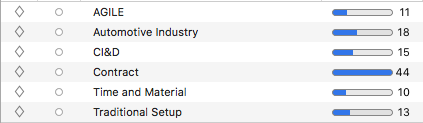
\includegraphics[width=\columnwidth]{figure/ss_CodeGroup6.png}
%\caption{Cultural change toward adopting more open or agile contracts for inter-organisational CI\&D}
%\label{fig:towardsAgile}
%\end{figure}

\noindent {\bf F7.1: Flexible contracts favour inter-organisational collaboration.} The interviewees share the opinion that a more open (or flexible) contract would be healthier for the project and benefit inter-organisational collaboration: 

\begin{aquote}{Chief Engineer, Tier-1 supplier}
I would say that in this case Volvo wants to work in an agile manner. That requires also basically agile contract. This is not really the case. This is in many sense stopping some of the activities...
\end{aquote}
%\rog{We have two factors here: more open transparency policy and being in the same office. It hard from the interviews to see which one has the largest effect:- Both seems to give positive results. Them main problem is that the contract stops both activities and transparency. Here we have several quotes against fix-prices, however, I don't know if this kind of quotes fit here, such as:
%
%Question: Do you feel that there are constrains imposed by the contract now the project is ongoing?
%
%Quote: Yes, I would say that in this case Volvo wants to work in an agile manner. That requires also basically agile contact. This is not really the case, This is in many sense stopping some of the activities...."
%
%}


Although some of the project members from both customer and supplier companies are not fully aware of the contract details, they do share the feeling of being restricted. 
%
%\begin{aquote}
%...the customer needs to know that when you put in new features in a high ranker than we need to take others out. You change the scope of the project and that is going to cost the supplier. The supplier is going to track this and are making losses. I have seen it happen before, so. But regarding CI, it is like any other project.
%\end{aquote}
%
They believe that strict contracts conflict with an agile way of working instead of supporting it, and suggest to adopt more flexible contracts, instead, also referred to as Time and Materials (T\&M) contracts\footnote{According to a T\&M contract, the contractor is being billed per hour regardless of the software project duration. If any additional features have to be developed the supplier charges just for the time spent by its employees working on a certain set of tasks [en.wikipedia.org]. This brings high flexibility to accommodate projects with evolving requirements, but also high uncertainty about the related costs.}. 
The interviewees agree that a T\&M contract allows for a better adaptation to project changes, distribution of resources, and it creates shared ownership otherwise hindered by traditional contracts:

\begin{aquote}{System Lead, Tier-1 supplier}
[...] it is possible in an agile world to do this differently, but the preferred way would be not to buy content [...] %, but today commercial contract is that bought a certain content. 
It would be better if they buy a certain number of engineering hours.
\end{aquote}

They also argue in favour of a combination of a fixed price and T\&M contract, where stakeholders would agree on the product and cost estimation, but maintain high-flexibility on how to produce it. This combination fulfils the need for flexibility and agility, but also better quality for the customer:

\begin{aquote}{Open Source and Community manager, Tier-1 supplier}
%I think it would be a more shared ownership when it was a full time and material work rather than contract. Because there need to be some checkpoints. 
I think there are so many unknowns in this project, but [the supplier company] is building a platform out of this project as well. So they are taking part of the risk here. The risk is on both side, but I think an agile project, a full agile project would be better. Then we could get to a situation earlier with quality.
\end{aquote}

All interviewees made it clear that good collaboration between their companies is important from a legal and contractual perspective to support inter-organisational CI\&D:

\begin{aquote}{Open Source and Community manager, Tier-1 supplier}
a looser contract would be better and healthier for the project. I know Volvo Cars has its time schedule, you can fix the time, but then it is the costs and functionalities that float and lead into more agile contract.
\end{aquote}


% To preserve an open approach to the project, a product manager at a software development company suggests a combination of an agile and fixed price contract by creating project branches to avoid overhead in the main project.

\noindent {\bf F7.2: Contracts ease negotiation.} For a customer it is (still) more comfortable to work with contracts because one has more leverage and binds the supplier to pre-defined deliverables and deadlines. A Volvo Cars manager %involved in a RFQ projects, 
further states that it is hard for suppliers to negotiate with a T\&M or other flexible contracts, and that traditional contracts make it easier competing with other suppliers.

% Accordingly, we elicit the following possible answers to proposition 6:

% \begin{itemize}
% \item Cross-organisational CI\&D benefits from a more open collaboration among companies, such as information sharing and adaptation to project changes. A strict contract is an impediment for this way of working related to cross-organisational CI\&D.
% \item A strict contract is an impediment for cross-organisational CI\&D. Although there is no direct connection between a strict contract and cross-organisational CI\&D, the way of working related to this method benefits from an open or agile contract.
% \item Cross-organisational CI\&D is possible with a strict contract, but synergy effects, i.e. collaboration and flexibility, are in effect when supported by an agile contract. By taking the synergy effects into account, a strict contract can be an impediment for Cross-Organisational CI\&D. An agile contract is difficult for a RFQ due to the open and uncertain characteristics of the contract.
% \end{itemize}

\vspace{.2cm}
\subsubsection{Proposition 8: Standards and processes, based on industry-wide data and process standards benefit inter-organisational CI\&D}

%This proposition challenges the interviewees to experience the effects of industry-wide standards and processes in a inter-organisational setting where companies work together in software engineering projects using CI\&D. 
The interviewees were asked if they use industry-wise standards, and whether they find them beneficial for information sharing, which is important for inter-organisational CI\&D. The automotive industry is participating in various open source projects (e.g. AUTOSAR and GENIVI) and attempts to be good open-source citizens:

\begin{aquote}{Open Source and Community manager, Tier-1 supplier}
We are trying to be a good open-source member by also upstreaming strategies, especially around GENIVI and Yocto. Here we find issues or improvements in the tools and we try to pass them back what we can. That is one of the strategies of [the company] to work more open towards the open-source community...% as a give and receiver. We are working on that.
\end{aquote}

And also:

\begin{aquote}{Open Source and Community manager, Tier-1 supplier}
Open source is a very strong area related to CI\&D [...]. The tools are open source and the automotive industry is trying to keep this an open-source as possible. There are some weak areas, like code coverage tools. They are very weak, unfortunately, so we have to use commercial tools for that.
\end{aquote}

This development also enables companies to hire new employees easier, because open-source knowledge is more common than knowledge of proprietary technology.


The interview results {\bf support the proposition}: industry standards and open-source projects allow a common language and shared knowledge, therefore, benefits information sharing, which is important for inter-organisational CI\&D. This answer to proposition 8 is deduced from the following findings.

\noindent {\bf F8.1: Beneficial for information sharing.} The industry standards and open-source projects allow a common language (i.e. AUTOSAR framework) and shared knowledge between project members; this improves communication and information sharing.

\noindent {\bf F8.2: Maturity and management.} It is important for the success and adoption of open-source projects and standards by stakeholder in the automotive industry, that these are highly controlled by one person, group or organisation. The maturity is also a crucial factor for the success or failure of an industry standard or open-source project.



\subsection{Summary of the findings and challenges}\label{sec:findings_RQs}

In this section we summarize the findings and highlight the main challenges while giving an answer to the research questions.


\paragraph*{RQ1: What are the risks and/or benefits of increasing inter-organisational transparency?} Inter-organisational transparency is not a necessary condition for inter-organizational CI\&D. However, transparency is considered positive and creates positive synergy effects in terms of efficiency, trust, and mutual understanding while avoiding useless stressful situations. Transparency is also considered positive in terms of increasing the overall project quality. 
There exist strategies to facilitate sharing inter organizations, however, the automotive industry experiences difficulties to share information, and manage responsibilities and IPR.
\paragraph*{RQ2: Is there a lack or overload of information that is exchanged across organizations?}  Increased transparency among organizations leads to much more information available to project members. In our pilot project participants feel that they have the information needed. However, they are missing a holistic project overview. This ``big picture" could be beneficial for all stakeholders and can increase project efficiency and quality. Information overload in terms of frequency of updates is not considered a problem if the information exchanged is precise, i.e. supply and demand of information correspond.
\paragraph*{RQ3: Are contracts an impediment for scaling agility across company boundaries, and 
are industry-wide standards and processes shared among organizations an enabler?}  Strict contract-based collaboration is an impediment for inter-organisational CI\&D. More flexible contracts will bring benefits to inter-organizational collaborations. However, contracts facilitates negotiations between different organizations. Industry-wide standards and processes that are shared among organizations promote collaborations, knowledge sharing, and communication. Open-source initiatives help in the same direction and facilitate also the hiring process since people are already skilled. However, open-source projects should be mature enough and the management of the project should be clearly controlled by a person, team, or organization.
%\end{itemize}


The biggest challenges identified in our study are: 

%\begin{itemize}
\paragraph{Challenge 1} The automotive industry experiences difficulties to share information in the ecosystem, as well as to manage responsibilities and IPRs. 
\paragraph{Challenge 2} When the collaboration between different organizations is regulated though more ``open-contracts", it is not obvious  how to manage negotiations and responsibility sharing. It is also difficult to evaluate offers from different suppliers, and, from the supplier point of view, to compete transparently with other suppliers. 
\paragraph{Challenge 3} Means and strategies to share a ``big picture" of the project among the different stakeholders should be identified. A holistic view of the project could be beneficial for all stakeholders and can increase project efficiency and quality. 
%\end{itemize}




%\rog{
%Hopefully, this will be the last quote. I just found this quote very interesting, it is about culture. Don't know how we could use it, maybe in a discussion or in our next paper:- 
%I will try not to add any more quotes now!
%
%Question: How do you experience the relationships between the members in this project? You mentioned that the trust is increasing.
%
%Quote: "It is always difficult to merge different organisations and cultures. Everybody in Delphi understands what needs to be done when we have a critical delivery or we have problems. Everybody understands certain rules within the company, for example, going home earlier on a Friday. You need to help out and support your colleagues. Due to this merge, we have new team members from Volvo or other 3rd party member. They don’t have the same rules in their cultures. Sometimes these other people leave earlier on Friday than Delphi people. This is of course an example and so are there more examples of differences in cultures of organisations. This could be positive or negative, not always negative of course. Also differences in workplaces, nearby facilities, such as restaurant, can have an effect on the members, so psychical elements can also influence each other. The change in culture or workplace can be either positive or negative for current or new team members. This is important to keep in mind when you merge organisations. If I need to ask my people to do overtime at the office, it is easier for me than when I ask this of an employee of the customer. I have to go to the customer and their manager and see if we can arrange something. This is also one of the many examples."
%
%
%
%}


%\pat{Add a summary and draw some conclusions}

%\begin{table}[htb]
%\centering
%\begin{tabular}{|c|c|c|c|}\hline
%{\bf Res. Quest. 1} & {\bf Res. Quest. 2} & {\bf Res. Quest. 3} & {\bf Res. Quest. 4}\\ \hline
%F3.3 & F2.1 & F3.1 & F9.1\\ \hline
%F6.2 & F2.2 & F3.2 & F9.2\\ \hline
%		 & F4.1 & F4.1 &\\ \hline
%		 & F4.2	& F6.2 &\\ \hline
%		 & F5.1 & F7.1 &\\ \hline
%		 & F6.1 & F8.1 &\\ \hline
%		 & 			& F8.2 &\\ \hline		
%\end{tabular}
%\caption{Mapping between research questions and findings}
%\label{tab:mapping}
%\vspace{-.4cm}
%\end{table}



% {\bf Industry Perspective.} 
% To preserve an open approach to the project, a product manager at a software development company suggests a combination of an agile and fixed price contract by creating project branches to avoid overhead in the main project.
%
%(Y)
% {\bf Maturity.} The automotive software ecosystem needs to adapt to the needs from the stakeholders. The industry is not mature enough, but is improving to adopt cross-organisational Continuous Integration and Deployment.
% Yes: Johnny Karlsson, Darrel Cullen, Lars Mattson, Petter Molder, Jacob Juul, Matti Larborn, 
% No: Anders Lindbom, Michael Svenstam, Mattias Almljum